\documentclass[article,12pt]{article}

\usepackage[utf8]{inputenc}
\usepackage{amssymb, amsfonts,amsthm}
\usepackage[fleqn]{amsmath} % Math packages
\numberwithin{equation}{section}
\usepackage{listings}
\usepackage[top=1in, bottom=1in, left=1in, right=1in]{geometry}
%\usepackage[T1]{fontenc} % Use 8-bit encoding that has 256 glyphs
%\usepackage{fourier} % Use the Adobe Utopia font for the document - comment this line to return to the LaTeX default
\usepackage[english]{babel} % English language/hyphenation
\usepackage{enumerate}
\usepackage[usenames,dvipsnames]{color} % Required for custom colors
\usepackage{listings} % Required for insertion of code
\usepackage{courier} % Required for the courier font
\usepackage{tikz} 
\usepackage{sectsty}
\usepackage{multicol} % Required for multiple columns
%\usepackage{tabu} % Option for Table Construction
\usepackage{epigraph} 
\setlength{\epigraphwidth}{\textwidth}
\usepackage{hologo}
\usepackage[font=small,labelfont=bf]{caption} % Specifying Captions
\usepackage{multirow} % TAbles
\usepackage{changepage} % Change margins



\usepackage{blindtext}
\usepackage{setspace} % Spacing
\usepackage{csquotes}% Recommended
\usepackage{psvectorian} % Cool ornaments

\usepackage{hyperref} % hyper links
\hypersetup{
	colorlinks=true,
	linkcolor=blue,
	filecolor=magenta,      
	urlcolor=cyan,
	pdftitle={Prospectus},
	pdfpagemode=FullScreen,
	citecolor= black
}

\urlstyle{same}


\renewcommand{\baselinestretch}{1.5} % Spacing

\usepackage[style = numeric, sorting = none, backend=biber]{biblatex}
\addbibresource{references.bib}

\usepackage{graphicx}
\graphicspath{{figs/}} %Setting the graphicspath


\begin{document}

\begin{center}
Lab Report

Title: Lab1\\
Notice: Dr. Bryan Runck\\
Author: Rob Hendrickson\\
Date: 11/02/2022\\~\\

Repository: \url{https://github.com/RwHendrickson/GIS5571/tree/main/Lab02/Part_2}\\
Time Spent: 25 hours

\end{center}

\section*{Abstract}
In this lab, I created a walk-ability cost surface for the area around Minnesota's Whitewater State Park. The problem statement section provides contextual information and requirements for analysis. The input data section will describe the different datasets acquired in this exercise. The methods section includes detailed visual and textual descriptions of the workflow conducted. The results section will present some visualizations of the surfaces that were created. This report concludes with a discussion on the lessons learned and future directions of this work.


\section{Problem Statement}
The client of this project is a fictional character named Dory who lives on a farm near the borders of Olmsted, Wabasha, and Winona counties. She enjoys walking to the North Picnic area of Whitewater State Park from time to time. Her journey is often quite enjoyable, however, it can also be quite treacherous if she chooses the wrong route at the wrong time of year. Her largest concerns are muddy farm fields in the spring and water bodies if there isn't a bridge (or she has her waders). Otherwise, she just prefers the most gradual slope. On the following page is a map of her journey and a table of the requirements for the cost surface construction.

\begin{adjustwidth}{-.7in}{-.7in}
	\begin{center}
\fbox{ % Workflow
	\begin{minipage}{.9\linewidth}
		\begin{center}
			\begin{minipage}{\linewidth}
				\includegraphics[width=\linewidth]{DoryTrip}
			\end{minipage}
			\captionof{figure}{A map of the study area with trip origin, destination, and water highlighted.}
		\end{center}
	\end{minipage}
}
\end{center}
\end{adjustwidth}
{
	\scriptsize
	\begin{tabular}{|l|p{.12\linewidth}|p{.2\linewidth}|p{.1\linewidth}|p{.2\linewidth}|p{.2\linewidth}|p{.1\linewidth}|}
	\hline	& \textbf{Requirement} & \textbf{Defined As} & \textbf{(Spatial) Data} & \textbf{Attribute Data} & \textbf{Dataset} & \textbf{Preparation} \\ \hline
		1 &  Elevation, Water, and Bridges      &    Acquire and process LiDAR data                                                             & Points         &   Elevation \& Category (Water, ground, bridges, etc.)                                               & \href{https://resources.gisdata.mn.gov/pub/data/elevation/lidar/}{Minnesota Dept. of Natural Resources}                                                                                                                &       Navigated the API tree \\ \hline
		2 &  Fields       &    Acquire and select relevant land classification data                                                            & Polygons         &   Landcover Classification                                  &      \href{https://gisdata.mn.gov/dataset/biota-landcover-mlccs}{Minnesota Land Cover Classification System}                                                                                                         &   \\ \hline
		3 &  Rasterize      & Convert all vectors into a common raster format                                                            & Points and Polygons         &  elevation (integer), is\_water\_no\_bridge (boolean), is\_field (boolean)                                               &  Elevation points, Water and no bridge points, field polygons                                                                                                              &       \\ \hline
		4 & Slope & Calculate slope from elevation               &    Raster                                     &   Elevation (integer)                                                & Rasterized elevation                                                                                                                                                                                                        &             \\ \hline
		5 &  Standardize      & Ensure that all values are in a similar range with appropriate sign                                                           & Rasters         &  slope (float), is\_water\_no\_bridge (boolean), is\_field (boolean)                                               &         Rasterized slope, is\_water\_no\_bridge, and is\_field                                                                                                       &       Explored distribution of values \\ \hline
		6 & Weight                            & Compose weights combinations between the 3 rasters that sum up to 1 &                   &                                                  &                                                                                                                                           &             \\ \hline
		7 & Cost Surface & Utilize map algebra to construct a walk-ability surface using all weight combinations               &  Rasters                                       &  standardized slope, standardized is\_water\_no\_bridge, standardized is\_field                                                 &                                                                                                                                                                                                         &             \\ \hline
		8 & Uncertainty Analysis & Compare cost surfaces to Dory's preferences              &    Rasters                                     &  Walk-ability Cost                                                 &                                                                                                                                                                                                         &             \\ \hline      
	\end{tabular}
\captionof{table}{Project requirements}}

\section{Input Data}
The data acquired from the Minnesota Department of Natural Resources (MnDNR) were 20 LiDAR tiles from Wabasha, Winona, and Olmsted counties. The full list of tiles is in figure 2 and were determined using each county's respective file title, \texttt{tile\_index\_map.pdf}. These tiles contain geographic information, classification (water, ground, bridge, vegetation, etc), and elevation. Information acquired from Minnesota Land Cover Classification System (MLCCS) contained polygons with classifications based on the MLCCS coding scheme. Their API links can be found in table 2. \vspace{.5in}

\begin{adjustwidth}{-.3in}{-.3in}
\begin{multicols}{2}

\fbox{ % Tilelist
	\begin{minipage}{.6\linewidth}
		\begin{center}
			\begin{minipage}{\linewidth}
				\includegraphics[width=\linewidth]{tilelist}
			\end{minipage}
			\captionof{figure}{Full list of LiDAR tiles in the format (county, tile id)}
		\end{center}
	\end{minipage}
}\\

{
	\scriptsize
	\begin{tabular}{|l|p{.2\linewidth}|p{.2\linewidth}|p{.4\linewidth}|}
	& \textbf{Title}                              & \textbf{Purpose in Analysis}     & \textbf{Link to Source} \\ \hline
	1 & MnDNR LiDAR Tiles & Determining location of water \& bridges, calculating slope & \url{https://resources.gisdata.mn.gov/pub/data/elevation/lidar/county/}        \\                 
	2 & MLCCS Land Cover Classifications     & Determining location of fields & \url{https://resources.gisdata.mn.gov/pub/gdrs/data/pub/us_mn_state_dnr/biota_landcover_mlccs/shp_biota_landcover_mlccs.zip}                                                            
\end{tabular}
\captionof{table}{Data Sources}}
\end{multicols}

\section{Methods}
\end{adjustwidth}

\fbox{ % Workflow
	\begin{minipage}{\linewidth}
		\begin{center}
			\begin{minipage}{\linewidth}
				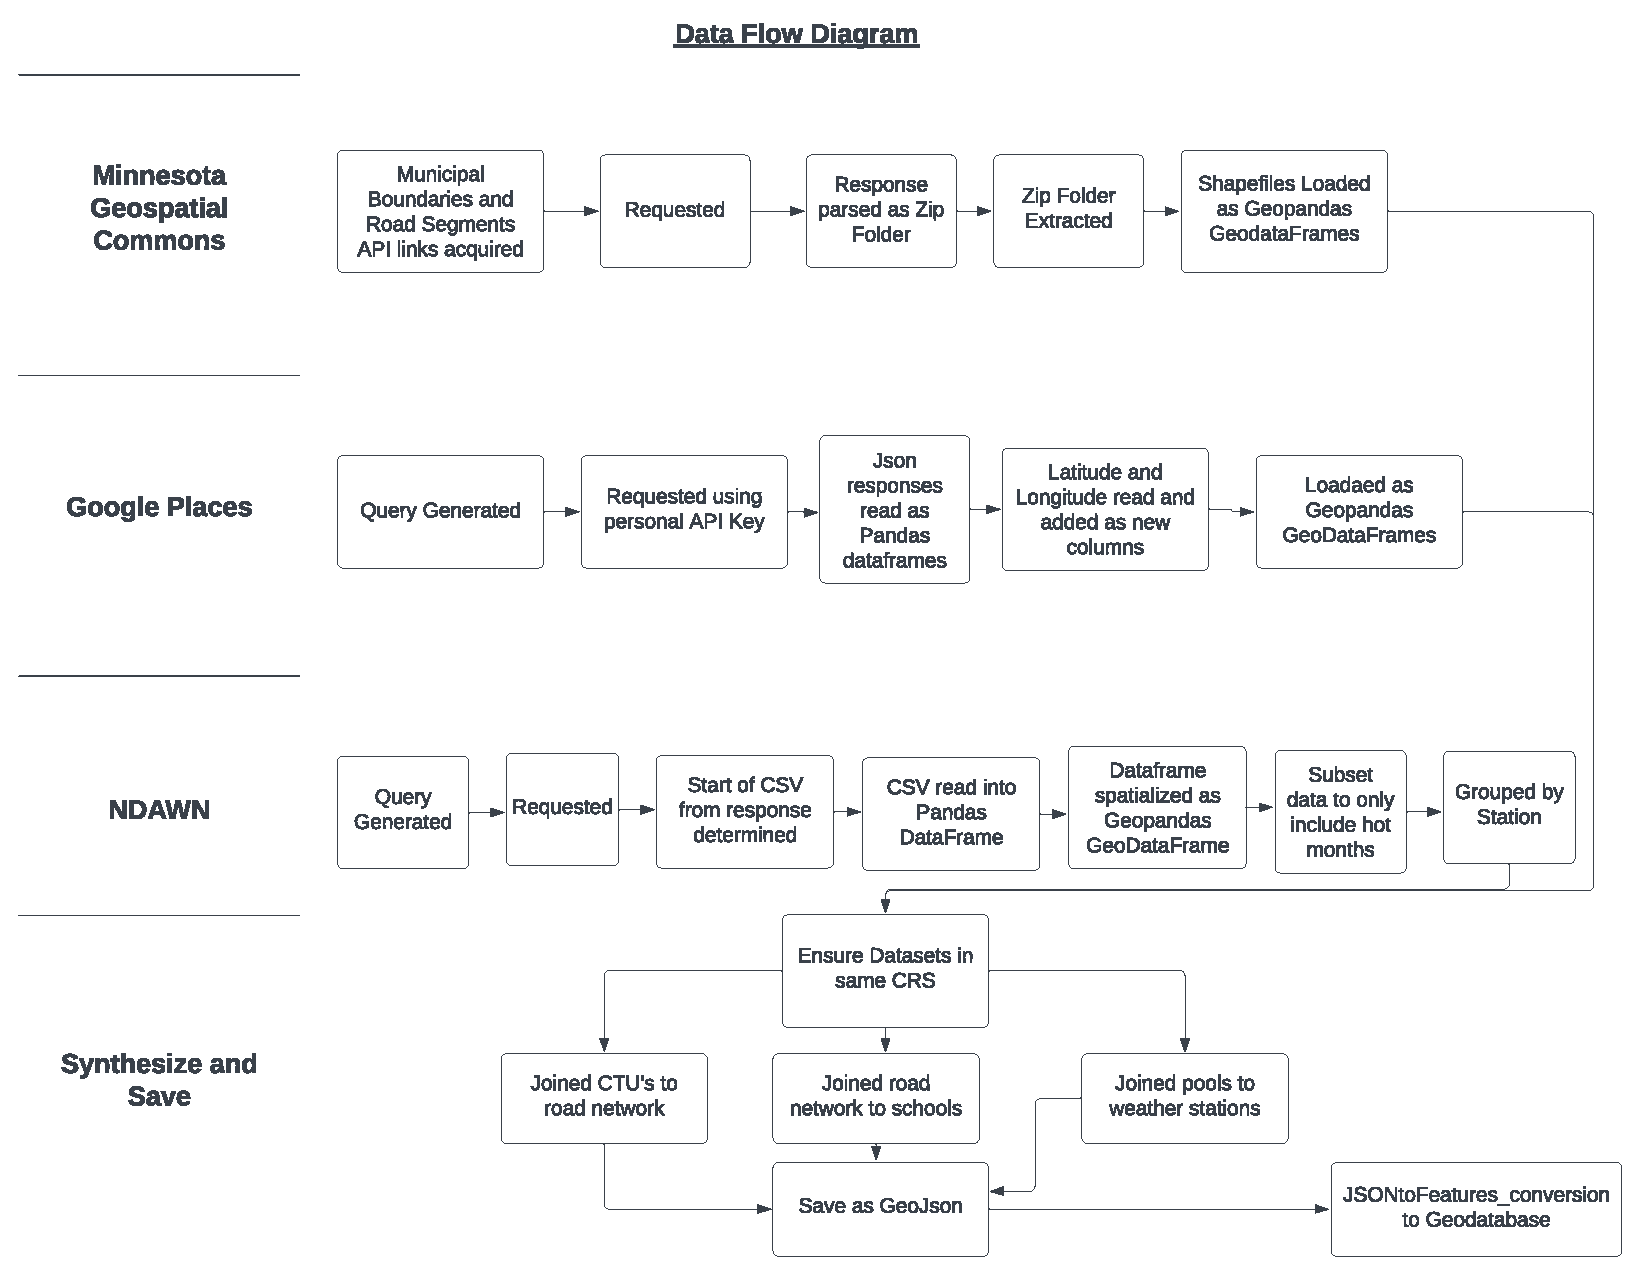
\includegraphics[width=\linewidth, height=.75\paperheight]{WorkFlow}
			\end{minipage}
			\captionof{figure}{Detailed Workflow}
		\end{center}
	\end{minipage}
}\\

\subsection{Data Input/Output}

\subsubsection{MnDNR}

To diagnose which LiDAR tiles were needed from MnDNR, the tile index maps were consulted from each county. An example of this map can be found here: \url{https://resources.gisdata.mn.gov/pub/data/elevation/lidar/county/winona/tile_index_map.pdf}. This list of tiles was iterated over and their respective \texttt{.laz} files were requested and written to disk. These files were decompressed into \texttt{.las} files utilizing Arcpy's ConvertLas function. Code to accomplish these tasks is provided in figures 4 and 5.

\begin{adjustwidth}{-.8in}{-.8in}
\begin{multicols}{2}
	\fbox{
		\begin{minipage}{.95\linewidth}
				\begin{center}
						\begin{minipage}{1\linewidth}
								\includegraphics[width=\linewidth]{downloadlaz}
							\end{minipage}
						\captionof{figure}{Iteratively interfacing with MnDNR's API}
					\end{center}
			\end{minipage}
	}\\
	\fbox{ 
		\begin{minipage}{.95\linewidth}
			\begin{center}
				\begin{minipage}{1\linewidth}
					\includegraphics[width=\linewidth]{convertlaz}
				\end{minipage}
				\captionof{figure}{Iteratively converting \texttt{.laz} files to \texttt{.las} files}
			\end{center}
		\end{minipage}
	}\\
\end{multicols}
\end{adjustwidth}

Once the files were in a \texttt{.las} format, they could be accessed with the Python library, \href{https://laspy.readthedocs.io/en/latest/index.html}{\texttt{laspy}}. The library claims to work with \texttt{.laz} files but it didn't work with my version. The extent of all the tiles was ascertained with the code in figure 6. This information was used to create a template raster for analysis (see section 3.2). It should be noted that the \texttt{.las} units are in centimeters.

\fbox{ 
	\begin{minipage}{.95\linewidth}
		\begin{center}
			\begin{minipage}{1\linewidth}
				\includegraphics[width=\linewidth]{getextent1}
				\includegraphics[width=\linewidth]{getextent2}
			\end{minipage}
			\captionof{figure}{Getting the extent of all \texttt{.las} tiles}
		\end{center}
	\end{minipage}
}\\

\subsubsection{MLCCS}

Land cover from MLCCS was accessed through the Minnesota Geospatial Commons's API. This link can be found in table 2. A zip file was downloaded and the shapefile within titled, \texttt{landcover\_minnesota\_land\_cover\_classification\_system.shp}, was read into Geopandas. Here it was clipped to the extent of the template raster (see section 3.2) and selected for the classification, 22 (agricultural land). This selected GeoDataFrame was saved in a \texttt{.geojson} format. The code that clips, selects, and saves is provided in figure 7.




\begin{adjustwidth}{-.7in}{-.7in}
	\fbox{
	\begin{minipage}{1\linewidth}
		\begin{center}
			\begin{minipage}{1\linewidth}
				\includegraphics[width=\linewidth]{clip}
			\end{minipage}
			\\
			\begin{minipage}{1\linewidth}
				\includegraphics[width=\linewidth]{selectsave}
			\end{minipage}
			\captionof{figure}{Clipping, selecting, and saving the land cover dataset.}
		\end{center}
	\end{minipage}
}\\
\end{adjustwidth}

\subsection{Creating Raster Template}

Upon identifying the extent of the \texttt{.las} files, the height and width of the study was computed. These were used to calculate dimensions of a regular grid of 10 meter resolution for the space. This grid was saved in both a Geotiff raster format and numpy mgrid. The code that executes these operations is in figures 8 - 11. \newpage

\begin{adjustwidth}{-.8in}{-.8in}
	\begin{multicols}{2}
		\fbox{
			\begin{minipage}{.95\linewidth}
				\begin{center}
					\begin{minipage}{1\linewidth}
						\includegraphics[width=\linewidth]{getdimensions}
					\end{minipage}
					\captionof{figure}{Calculating width and height of study extent.}
				\end{center}
			\end{minipage}
		}\\
		\fbox{ 
			\begin{minipage}{.95\linewidth}
				\begin{center}
					\begin{minipage}{1\linewidth}
						\includegraphics[width=\linewidth]{createraster}
					\end{minipage}
					\captionof{figure}{Computing number of cells in each dimension for raster.}
				\end{center}
			\end{minipage}
		}\\
		\fbox{
			\begin{minipage}{.95\linewidth}
				\begin{center}
					\begin{minipage}{1\linewidth}
						\includegraphics[width=\linewidth]{save_geotiff}
					\end{minipage}
					\captionof{figure}{A function for saving a geotiff file.}
				\end{center}
			\end{minipage}
		}\\
		\fbox{ 
			\begin{minipage}{.95\linewidth}
				\begin{center}
					\begin{minipage}{1\linewidth}
						\includegraphics[width=\linewidth]{savetemplate}
					\end{minipage}
					\captionof{figure}{Saving the template raster.}
				\end{center}
			\end{minipage}
		}\\
	\end{multicols}
\end{adjustwidth}

\subsection{Aggregate and Rasterize}

\subsubsection{Elevation}

To get a full elevation raster, the \texttt{.las} files were iterated over. Each was read using the \texttt{laspy} library and rasterized using Rasterio's \texttt{features.rasterize} function. This function does not have an average values option when merging points into a cell, so their elevations were sorted in ascending order and the \href{https://rasterio.readthedocs.io/en/latest/api/rasterio.enums.html#rasterio.enums.MergeAlg}{merge algebra}, 'REPLACE' was used. This effectively burned the largest \texttt{.las} point value for each cell into the template raster's format and saved it as a geotiff. Once complete, all intermediate rasters were summed up and overlapping cells were averaged. Code that accomplishes these tasks are in figures 12 and 13. This final raster was saved as a geotiff called, \texttt{full\_elevation.tif}.
\newpage
		\fbox{
			\begin{minipage}{.95\linewidth}
				\begin{center}
					\begin{minipage}{1\linewidth}
						\includegraphics[width=\linewidth]{rasterizeelev}
					\end{minipage}
					\captionof{figure}{Iteratively rasterizing the \texttt{.las} files.}
				\end{center}
			\end{minipage}
		}\\
	\begin{center}
		\fbox{ 
			\begin{minipage}{.6\linewidth}
				\begin{center}
					\begin{minipage}{1\linewidth}
						\includegraphics[width=\linewidth]{loadintelevs}
						\includegraphics[width=\linewidth]{mergeelev}
					\end{minipage}
					\captionof{figure}{Merging intermediate elevation rasters.}
				\end{center}
			\end{minipage}
		}
	\end{center}

\subsubsection{Water and Bridges}

The \texttt{laspy.read()} objects have a classification attribute which yields a numpy array of each point's classification. 2 indicated ground, 9 indicated water, and 14 indicated bridge decks. There is also 8 (model keypoint) and 12 (overlapping points) which could be utilized in future projects. No bridge decks were identified in any of the MnDNR's \texttt{.las} files, but it was assumed that breaks in the water points were bridges. After selecting only water classified points, a similar process to that in section 3.3.1 was conducted to rasterize the points to the template raster where the value burned was -1 if water and 0 if not. This final raster was saved as a geotiff called, \texttt{full\_water.tif}.

\subsubsection{Fields}

The fields geojson was loaded as a Geopandas Geodataframes and rasterized using the same process as 3.3.1 (without the iteration) and saved as \texttt{rasterized\_fields.tif}.

\subsection{Transform and Normalize Costs}
\begin{adjustwidth}{0in}{-.8in}
	\begin{multicols}{2}
Each of the final rasters, \texttt{full\_elevation.tif}, \texttt{full\_water.tif}, and \texttt{rasterized\_fields.tif} were transformed and/or normalized to align with Dory's preferences. Negative values indicate a cost (which all variables are) and all magnitudes were between 0 and 1. They were saved in the same format as the template using the function in figure 14.\\ 

~\columnbreak
\fbox{
	\begin{minipage}{.9\linewidth}
		\begin{center}
			\begin{minipage}{1\linewidth}
				\includegraphics[width=\linewidth]{savegeotifftotemplate}
			\end{minipage}
			\captionof{figure}{A function to save an array to a template raster.}
		\end{center}
	\end{minipage}
}

	\end{multicols}
\end{adjustwidth}
\subsubsection{Slope}

To calculate slope, first the gradient was calculated using Numpy's gradient function on the elevation (in meters) and then this was converted into slope degrees (see code in figure 15). The distribution of values was found to be heavily tailed (see figure 16) so it was transformed using $log_{10}$ which produced a multimodal distribution. The logged slope values were further transformed by shifting values by the minimum value and multiplied by -1. Finally they were normalized by the maximum value to achieve the "standardized" slope cost surface (code in figure 17, distribution in figure 18). 

\begin{adjustwidth}{-.8in}{-.8in}
	\begin{multicols}{2}
		\fbox{
			\begin{minipage}{.95\linewidth}
				\begin{center}
					\begin{minipage}{1\linewidth}
						\includegraphics[width=\linewidth]{getslope}
					\end{minipage}
					\captionof{figure}{Computing slope degrees.}
				\end{center}
			\end{minipage}
		}\\
		\fbox{ 
			\begin{minipage}{.95\linewidth}
				\begin{center}
					\begin{minipage}{1\linewidth}
						\includegraphics[width=\linewidth]{slopedist}
					\end{minipage}
					\captionof{figure}{Distribution of slope degree values.}
				\end{center}
			\end{minipage}
		}\\
		\fbox{
			\begin{minipage}{.95\linewidth}
				\begin{center}
					\begin{minipage}{1\linewidth}
						\includegraphics[width=\linewidth]{transformslope}
					\end{minipage}
					\captionof{figure}{Transforming and normalizing slope degree.}
				\end{center}
			\end{minipage}
		}\\
		\fbox{ 
			\begin{minipage}{.95\linewidth}
				\begin{center}
					\begin{minipage}{1\linewidth}
						\includegraphics[width=\linewidth]{finalslopedist}
					\end{minipage}
					\captionof{figure}{Final distribution of transformed and normalized slope.}
				\end{center}
			\end{minipage}
		}\\
	\end{multicols}
\end{adjustwidth}

\subsubsection{Water and Fields}

The water and fields boolean rasters were just ensured to be -1 (if field or water) and 0 otherwise. 
\newpage
\subsection{Cost Surface Computation}

	All weights between costs were standardized to be between 0 and 1. Weights combinations (by increments of 0.1) were generated using code in figure 19. These weights combinations were iterated through and multiplied by the respective cost rasters. The resulting summation of the weighted rasters was saved with the title format \texttt{\_\_S-\_\_W-\_\_F-Cost\_Surface.tif} where the blanks coincide with the percentage that raster was weighted (S = Slope, W = Water, F = Fields). This code can be seen in figure 20.
	
\begin{adjustwidth}{-.8in}{-.8in}
\begin{multicols}{2}
	\fbox{ 
		\begin{minipage}{.95\linewidth}
			\begin{center}
				\begin{minipage}{1\linewidth}
					\includegraphics[width=\linewidth]{weightscombos}
				\end{minipage}
				\captionof{figure}{Creating weights combinations for cost surface creation.}
			\end{center}
		\end{minipage}
	}\\	
	\fbox{ 
		\begin{minipage}{.95\linewidth}
			\begin{center}
				\begin{minipage}{1\linewidth}
					\includegraphics[width=\linewidth]{costsurfacecomp}
				\end{minipage}
				\captionof{figure}{Iterating through weights combinations and saving resulting cost surfaces.}
			\end{center}
		\end{minipage}
	}


\end{multicols}
\end{adjustwidth}
\subsection{Uncertainty Analysis}

Select cost surfaces were visualized using matplotlib's pcolormesh plot to understand how varying the weights effected the cost surface. An example function that creates this type of visualization can be found in figure 21. 

\fbox{ 
	\begin{minipage}{.95\linewidth}
		\begin{center}
			\begin{minipage}{1\linewidth}
				\includegraphics[width=\linewidth]{sixplot}
			\end{minipage}
			\captionof{figure}{Function to plot six cost surfaces.}
		\end{center}
	\end{minipage}
}

\section{Results}

\begin{adjustwidth}{-.8in}{-.8in}
	\begin{center}
	\fbox{ 
		\begin{minipage}{.72\linewidth}
			\begin{center}
				\begin{minipage}{1\linewidth}
					\includegraphics[width=1\linewidth]{No Water Cost Surfaces}
				\end{minipage}
				\captionof{figure}{Cost Surfaces with no weight on water cost.}
			\end{center}
		\end{minipage}
	}\\
	\fbox{ 
		\begin{minipage}{.72\linewidth}
			\begin{center}
				\begin{minipage}{\linewidth}
					\includegraphics[width=1\linewidth]{No Field Cost Surfaces}
				\end{minipage}
				\captionof{figure}{Cost Surfaces with no weight on field cost.}
			\end{center}
		\end{minipage}
	}\\
	\fbox{ 
		\begin{minipage}{.72\linewidth}
			\begin{center}
				\begin{minipage}{\linewidth}
					\includegraphics[width=\linewidth]{50 Percent Weighted Slope Cost Surfaces}
				\end{minipage}
				\captionof{figure}{Cost Surfaces with 50\% weight on slope cost.}
			\end{center}
		\end{minipage}
	}\\
	\fbox{ 
		\begin{minipage}{.72\linewidth}
			\begin{center}
				\begin{minipage}{\linewidth}
					\includegraphics[width=\linewidth]{50 Percent Weighted Water Cost Surfaces}
				\end{minipage}
				\captionof{figure}{Cost Surfaces with 50\% weight on water cost.}
			\end{center}
		\end{minipage}
	}\\
	\fbox{ 
		\begin{minipage}{.72\linewidth}
			\begin{center}
				\begin{minipage}{\linewidth}
					\includegraphics[width=\linewidth]{50 Percent Weighted Field Cost Surfaces}
				\end{minipage}
				\captionof{figure}{Cost Surfaces with 50\% weight on field cost.}
			\end{center}
		\end{minipage}
	}\\
	\fbox{ 
		\begin{minipage}{.95\linewidth}
			\begin{center}
				\begin{minipage}{\linewidth}
					\includegraphics[width=\linewidth]{Seasonal Cost Surfaces}
				\end{minipage}
				\captionof{figure}{Proposed cost surfaces for each season.}
			\end{center}
		\end{minipage}
	}\\
\end{center}
\end{adjustwidth}

Visually the results appear to be accurate.

\section{Discussion and Conclusion}

In this lab I explored creating a cost surface using almost all open sourced code. 

Interfacing with the API's wasn't too difficult besides dealing with the cross-county \texttt{.laz} tiles and the tile index maps. I was a little disappointed that I couldn't get laspy to read the compressed\texttt{.laz} files, but I'm sure that this could be resolved with more time.

I have grown quite comfortable over the past year (and certainly more so after this lab) with utilizing Numpy and Rasterio to deal with rasters in Python. The largest concerns in this department were not having an option to average values when merging features into a raster cell and not having the snap to raster feature when rasterizing bridges (though I think this snap feature could be achieved with a little more time potentially using Geopandas' sindex.nearest method). Another insight from this stage in the project was that the classifications of the \texttt{.las} points could be used to aid in creating a more accurate surface (such as the model keypoints and overlapping points).

The fun in this lab really began when exploring the slope values across the study area. It was rather curious that the log transform of these values showed a multimodal distribution and it would be cool to categorize the slopes based on this insight (ie. a scale of 0 to 4 in difficulty). The cost surfaces were extremely cool visually (particularly when slope was involved) and the influence the weights had on the surface was another curiosity.

Take the interaction between field and slope (without water) for example. We can see that as we increase the weight of slope, the slope surface slowly materializes underneath the areas designated as fields. Looking at the interaction between two costs at a time led to some knowledge on each that informed the final seasonal cost surfaces. In spring we weighted water and fields higher and can see that this makes much of the southwest of the study area look unappealing as a route to Whitewater Park (except via roads). After the harvest, there may be many good routes through this area! It would be interesting to take these surfaces to the next level and find the most optimal routes. Maybe even do some random walks to get a feeling about the different options Dory has.

Upon completing this lab, I am much more confident with cost surfaces, rasters, and open sourced workflows for dealing with \texttt{.las} files and look forward to implementing these newfound skills into future projects!  

%\begingroup           % Ctrl T to uncomment
%\setstretch{1}
%\setlength\bibitemsep{12pt}  % length between two different entries
%\printbibliography
%\endgroup

\section*{Self Score}
\setstretch{.2}
\begin{tabular}{|p{.2\linewidth}|p{.2\linewidth}|p{.2\linewidth}|p{.1\linewidth}|}
	\hline
	\textbf{Category}            & \textbf{Description}                                                                                                                                                                                                                                                                                                                                              & \textbf{Points Possible} & \textbf{Score} \\ \hline
\vspace{.2in}\textbf{Structural Elements} & {\tiny All elements of a lab report are included (2 points each): Title, Notice: Dr. Bryan Runck, Author, Project Repository, Date, Abstract, Problem Statement, Input Data w/ tables, Methods w/ Data, Flow Diagrams, Results, Results Verification, Discussion and Conclusion, References in common format, Self-score}                                        & \vspace{.2in}28              &   \vspace{.2in}24    \\ \hline
	\vspace{.2in}\textbf{Clarity of Content}  & {\tiny Each element above is executed at a professional level so that someone can understand the goal, data, methods, results, and their validity and implications in a 5 minute reading at a cursory-level, and in a 30 minute meeting at a deep level (12 points). There is a clear connection from data to results to discussion and conclusion (12 points).} & \vspace{.2in}24              &  \vspace{.2in}20     \\ \hline
	\vspace{.2in}\textbf{Reproducibility}     & {\tiny Results are completely reproducible by someone with basic GIS training. There is no ambiguity in data flow or rationale for data operations. Every step is documented and justified.}                                                                                                                                                                     & \vspace{.2in}28              &     \vspace{.2in}28  \\ \hline
	\vspace{.2in}\textbf{Verification}        & {\tiny Results are correct in that they have been verified in comparison to some standard. The standard is clearly stated (10 points), the method of comparison is clearly stated (5 points), and the result of verification is clearly stated (5 points).}                                                                                                      & \vspace{.2in}20              &   \vspace{.2in}10   \\ \hline
	&                                                                                                                                                                                                                                                                                                                                                          & \vspace{.02in}100             &   \vspace{.02in}82     \\ \hline
\end{tabular}
\end{document}